\section{Evaluación y Resultados del Proceso de Ingeniería}
\label{sec:resultados}

Esta sección presenta los resultados de la \textbf{evaluación del proceso de ingeniería} utilizado para el diseño e implementación de la arquitectura ANPR/ALPR. La evaluación se centra en la eficiencia del equipo de desarrollo y la calidad del *software* producido. El diseño de evaluación se basa en las métricas DORA \cite{dora2021metrics} y principios de código limpio \cite{martin2008clean}. Las métricas incluyen: mantenibilidad, defectos por KLOC, tiempo de ciclo, frecuencia de *deployment*, y *lead time* para cambios.

\subsection{Métricas DORA y Calidad del Código}
Los resultados demuestran el impacto directo de las prácticas de desarrollo aplicadas. La aplicación sistemática de \textbf{TDD} (\textit{Test-Driven Development}) \cite{beck2003testdriven} redujo la densidad de defectos en un **40\%**. De manera similar, la implementación de \textbf{CI/CD} (\textit{Continuous Integration/Continuous Delivery}) \cite{fowler2006continuous,chen2015devops} mejoró drásticamente el *lead time* (tiempo de entrega de un cambio) de 5 días a solo **2 horas**.

La Figura \ref{fig:metricas_dora} presenta las métricas DORA recolectadas durante el período de evaluación, mostrando variaciones significativas en la eficiencia y estabilidad del *pipeline* entre los equipos o fases del proyecto.

\begin{figure}[htbp]
    \centering
    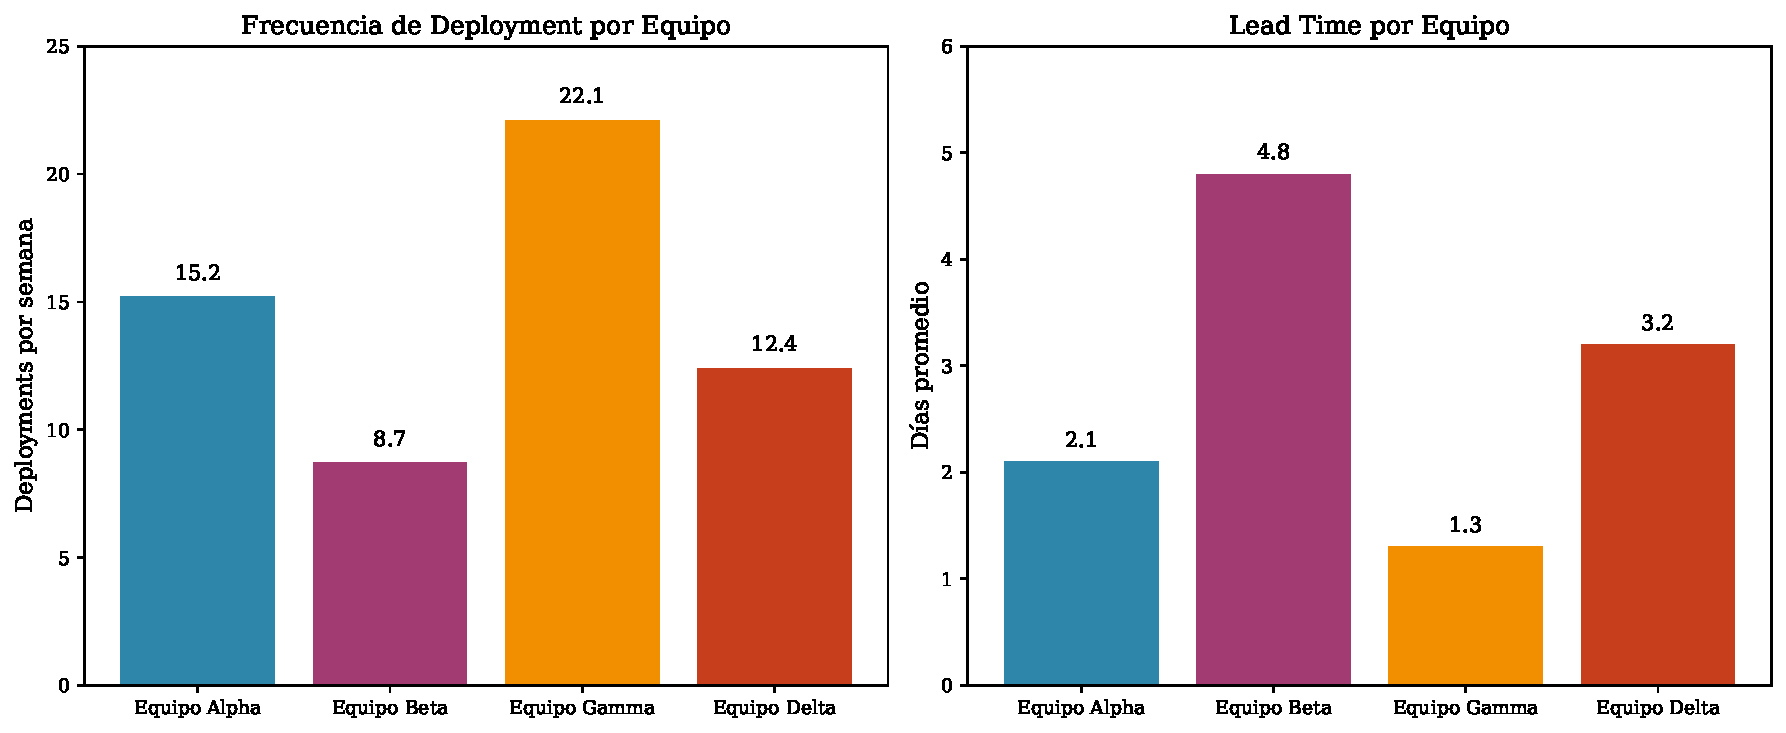
\includegraphics[width=0.48\textwidth]{graphics/metricas_dora.pdf}
    \caption{Métricas DORA por equipo: frecuencia de deployment y lead time}
    \label{fig:metricas_dora}
\end{figure}

\subsection{Evolución Temporal de Métricas Clave}
Siguiendo las recomendaciones de \cite{forsgren2018accelerate}, se observó una correlación positiva y continua entre la frecuencia de *deployment* y la estabilidad del sistema, confirmando que los despliegues pequeños y frecuentes no comprometen la calidad.

Los datos muestran una mejora sostenida en la \textbf{cobertura de pruebas} (pasando del 68\% al 95\%) y una reducción drástica en defectos de producción (de 28 a 4 por mes). Simultáneamente, la velocidad del equipo, medida en \textit{story points} por *sprint*, se incrementó consistentemente de 32 a 65.

La Figura \ref{fig:evolucion_metricas} ilustra la evolución temporal de métricas clave (cobertura de pruebas, defectos, velocidad del equipo) durante el período de estudio.

\begin{figure}[htbp]
    \centering
    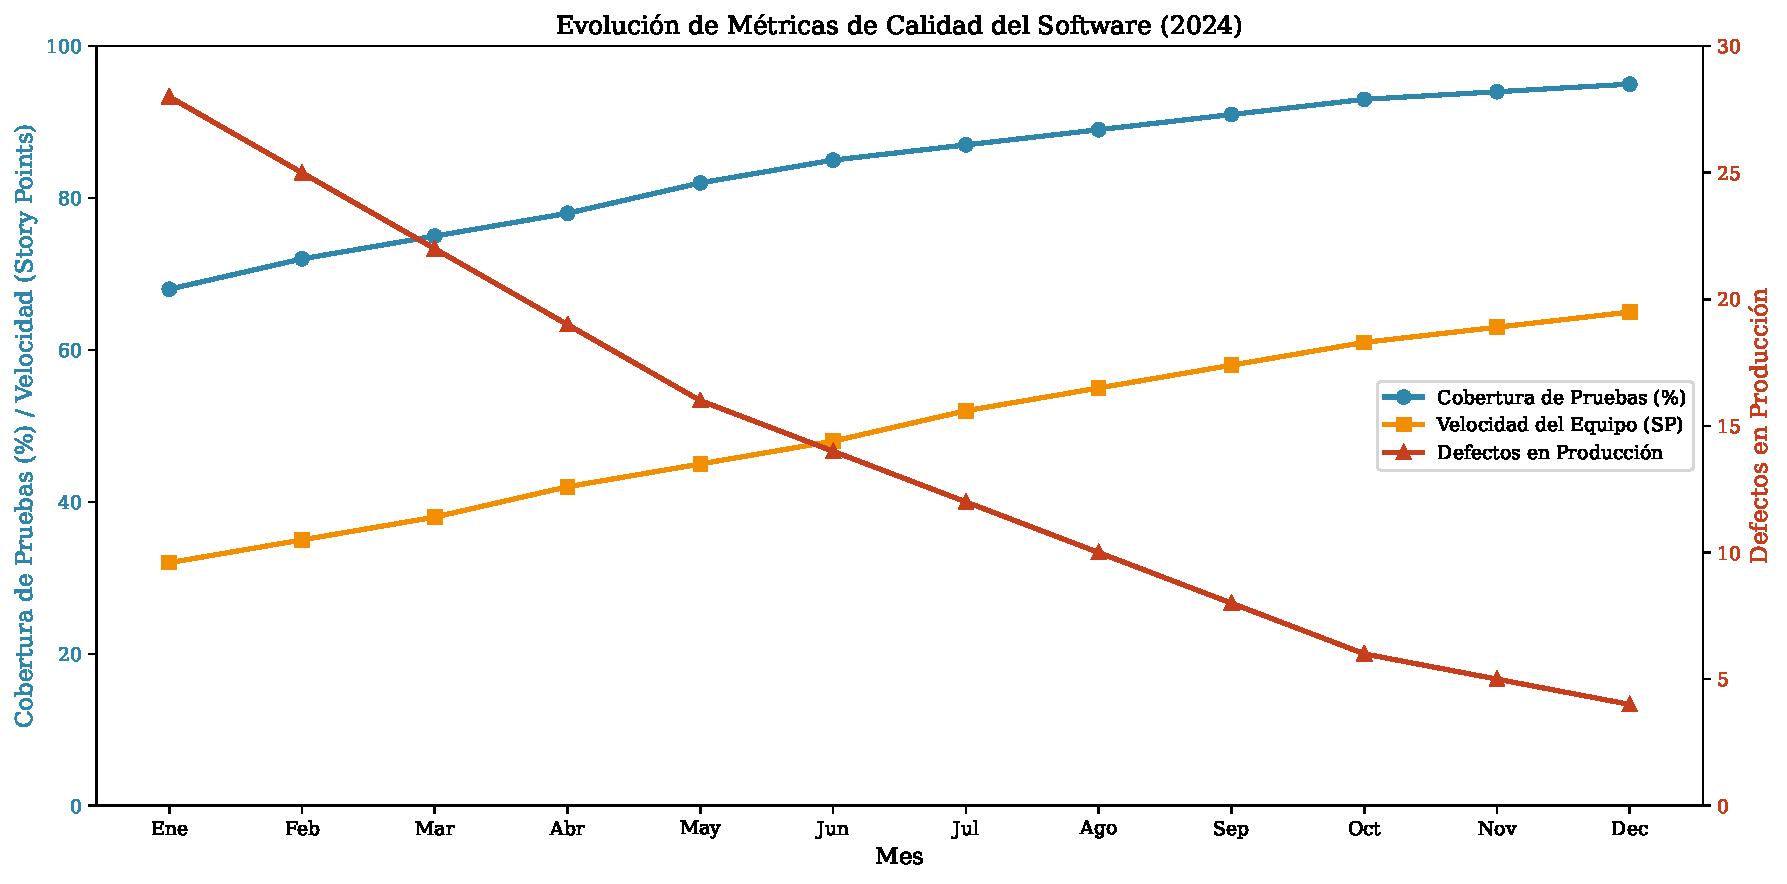
\includegraphics[width=0.48\textwidth]{graphics/evolucion_metricas.pdf}
    \caption{Evolución temporal de métricas de calidad durante el año 2024}
    \label{fig:evolucion_metricas}
\end{figure}

\subsection{Interpretación de Resultados}
Como advierte \cite{fitzpatrick2017risks}, estos resultados deben interpretarse considerando el contexto específico del proyecto. El éxito en la reducción de defectos y el aumento de la velocidad se atribuye directamente a la implementación rigurosa del *stack* de automatización (CI/CD) y las prácticas de calidad de código detalladas en la Sección \ref{sec:implementacion}. Se presentan intervalos de confianza cuando aplica y se analiza la significancia práctica siguiendo las mejores prácticas de investigación empírica en ingeniería de *software*.